\chapter{Einleitung}

Die vorliegende Ausarbeitung beschreibt den Aufbau, die Funktion sowie technische Hintergründe des "Audio reactive LED Strips".
Der vollständige Sourcecode ist im verlinkten GitHub Repository zu finden.

\section{Hardware und Funktion der Anwendung}
Für die Anwendung werden ein Raspberry Pi, ein LED-Streifen sowie ein Mikrofon mit Soundkarte und eine Sonos Musikanlage benötigt.
Auf dem Raspberry Pi wurde als Betriebssystem RaspberryOS installiert. Der in Python geschriebenen Sourcecode wird ebenfalls auf dem 
Raspberry ausgeführt. Die Netzwerkanbindung erfolgte via WLAN.
Um die LEDs des LED-Streifens anzusteuern wird ein Kabel an einen GPIO Pin des Raspberry PIs angeschlossen. Die Stromversorgung erfolgt über ein seperates Netzteil um
bei längeren Betrieb den Raspberry Pi nicht zu überlasten. Zusätzlich wird via USB eine Soundkarte an den Pi angeschlossen, welche das eingehenden Audio Signal an den Pi weiterleitet.
\\
Die Funktionalität der Anwendung lässt sich in zwei Modi unterteilen. Der erste Modus dient dazu, visuelle Effekte zu berechnen und auf den
LED-Streifen darzustellen während auf der Sonos Anlage Musik abgespielt wird. Die berechneten Effekte sind Abhängig von den vom Mikrofon 
erfassten Musik. Der zweite Modi ist aktiv sobald über den Fernseher Filme oder Serien geschaut werden und der Ton dieser über die bereits
erwähnte Sonos Anlage wiedergegeben wird. In diesem Modi soll der LED-Streifen konstant in einer Farbe leuchten. 
Wird weder ferngesehen noch Musik gehört wird der LED-Streifen abgeschaltet. Die Umschaltung zwischen den zwei Darstellungsmodi sowie das einschalten des LED-Streifens
erfolgt automatisch durch Abfrage von Parametern der Sonos Anlage.  

\section{Verwendete Technologien}
Die Anwendung wurde in der Skriptsprache Python in der Verson 3.9.7 erstellt. Eine Ausführung ist jedoch auch mit niedrigeren Versionsnummern bis Version 3.6 möglich.
Für die Ausführung werden verschiedene Standardmäßig nicht installierte Pakete benötigt. Als relevanteste Abhängigkeiten sind hier pyaudio, Sonos Controller (kurz SOCO) und neopixel zu erwähnen.
Pyaudio stellt verschiedene Funktionen zur Aufnahme, Verarbeitung und Speicherung von Audiosignalen zur Verfügung. Innerhalb dieser Anwendung wird es verwendet um 
die im Raum gespielte Musik aufzunehmen. Die SOCO Bibliothek ermöglicht Lautsprecher der Marke Sonos zu kontrollieren und deren Zustand (bspw. aktuell gespieltes Lied) 
auszulesen. Hierbei ist zu erwähnen das SOCO keine vollständige Implementierung für die Wiedergabe von TV-Inhalten implementiert. Wie mit dieser Einschränkung umgegangen wurde,
wird im Kapitel Realisierung erläutert.Die Bibliothek neopixel dient zur Ansteuerung der
LEDs. Sie bietet zum einen Funktionen um den Streifen in einer Farbe leuchten zu lassen, kann aber auch einzelne LEDs ansteuern.

\section{Struktur der Anwendung}
Um für dritte und spätere eventuelle Weiterentwicklungen die Übersichtlichkeit zu erleichtern wurde der Quellcode auf verschiedene Python Dateien aufgeteilt. 
Folgende Dateien sind Bestandteil der Anwendung:

\begin{itemize}
\item config.py - Konfigurationsdatei
\item led.py - LED-Funktionen
\item microInput.py - Aufnahme von Audiosignalen
\item TVStateEnum.py - Enumeration für Status der Sonos Anlage
\item wave2RGB.py - Funktionen zur Farbberechnung
\item main.py - Hauptdatei zur Ausführung
\end{itemize}

Die Ausführung der Anwendung erfolgt mithilfe der main Datei. Diese ruft einzelne Funktionen und Klassen der anderen Dateien auf und beinhaltet auch die Funktionalität der
Farbberechnung zu AudioSignalen. In der main Datei und auch in allen anderen Dateien werden wesentliche Konfigurationsparameter aus der zentralen Konfigurationsdatei bezogen.
Dies erleichtetert Entwicklern und Anwendern Änderungen vorzunehmen und zu konsistent zu testen. Im  folgenden soll der Ablauf der Ausführung und die technischen Hintergründe
erläuter werden.

\chapter{Programmablauf}
\section{Abfrage der Sonos Anlage}
Die Ausführung beginnt in der main Methode innerhalb der gleichnamigen Datei. Hier werden einige notwendige globale Variablen initialisiert und alle wesentlichen Methoden
aufgerufen. Das zentrale Element der Methode ist eine endlose Schleife. Innerhalb dieser Schleife wird in jedem Durchlauf der akutelle Zustand der Sonos Analge erfasst 
und ausgewertet um zu ermitteln welcher Modus im Moment gewünscht ist. Der Zustand wird in Form einer Variable des Typs TVStateEnum gespeichert. 
Diese beinhaltet Zustände für die Wiedergabe von Musik und TV-Audio sowie einen Pause Zustand. Diese Zustände werden im weiteren Programmablauf verwendet um festzustellen
welcher Modus aktuell ausgeführt wird und ob ein Moduswechsel erforderlich ist. Wie genau der Modus wechsel erfolgt, wird in den folgenden Kapitel beschrieben.

Die Abfrage der Sonos Anlage erfolgt über einen Aufruf der updateCurrentState Funktion. Diese fragt mithilfe der SOCO Bibliothek den Wiedergabestatus und
das akutell gespielte Lied ab. Durch diese Abfrage kann ermittle welcher Zustand der TVStateEnum zurückgegeben werden muss. 
Ein Sonderfall ist die Wiedergabe von Audioinhalten eines Fernsehers. Wie bereits in der Einleitung erwähnt implementiert SOCO diesen Fall nicht vollständig.
Wird ein solches Audiosignal wiedergeben wird keine Information über den akutell wiedergegeben Titel zurückgegeben, jedoch erkannt das Anlage aktuell Ton abspielt. 
Aus diesem Grund ist die Abfrage für in der zweiten Fallunterscheidung wie in der Abbildung 2.1 zu sehen entsprechend angepasst. Wurde nach der Status Abfrage
festgestellt das der akutelles Modus nicht gewechselt werden muss, wird der main Thread einige Sekunden pausiert. Durch diese Vorgehen können Abfragen ohne Mehrwert vermieden werden
und der Ressourcenverbrauch reduziert werden. 

\begin{figure}[ht]
    \centering
    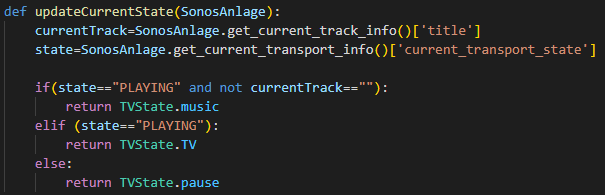
\includegraphics[scale=0.5]{UpdateCurrentState.png}
    \caption{Abfrage Sonos Anlage}
    \label{UpdateCurrentState}
\end{figure}

\section{Musikmodus}
\subsection{Musik Modus starten und beenden}
Der Musik Modus dient dazu passende Farben anhand des Audiosignals zu berechnen und auf dem LED-Streifen darzustellen. Jedoch ist es erforderlich, parallel zu der Verarbeitung
der Audiosignale, weiterhin den Status der Sonos Anlage zu beobachten um einen späteren erneuten Moduswechsel zu ermöglichen. Die Parallelität dieser Abfrage und der 
Audioverarbeitung wurde durch Multi Threading ermöglicht. Wird in den Musik Modus gewechselt wird ein neuer Thread (im folgenden Musik Thread genannt) gestartet,
welcher die Ausführung der nötigen Funktionen übernimmt. Der Main Thread prüft im Anschluss lediglich den Zustand der Sonos Anlage in regelmäßigen Intervallen. 
Wird im Main Thread ein erneuter Modus Wechsel erkannt, sendet er über eine Queue an den Musik Modus Thread eine Task welche die Terminierung über einen entsprechenden Handler
einleitet und die Task aus der Queue wieder entnimmt. Zu der Realisierung dieser Funktion sollte erwähnt werden, dass Python kein Mehrkern Multithreading unterstüzt. Daher
laufen die Threads nicht echt parallel auf unterschiedlichen Kernen. Für den gewünschten Zweck ist die vohrandene Implementierung jedoch hinreichend, da der Main Thread die meiste
Zeit wartend verbringt . Bei einer späteren Weiterentwicklung könnten statt eines zweiten Threads ein separater Prozess erzeugt werden, 
welcher die Ausführung der Funktion übernimmt. Dies würde eine parallele Ausführung ermöglichen und möglicherweise die Performance der Anwendung steigern.

\subsection{Audioaufnahme und Farbberechnung}
Die Aufnahme und Verarbeitung des Audiosignals beginnt mit dem starten des Musik Threads, sobald die Abfrage der Sonos Anlage das entsprechende Ergebnis produziert hat. 
Für die Aufnahme des Audiosignals wird in der Methode recordAudio zunächst ein Objekt der Klasse Rekorder erstellt, welche mithilfe der Pyaudio Bibiliothek 
Signale des Standardeingabegerätes des Raspberrys erfässt.
Im Konstruktor dieser Klasse werden verschiedene Parameter, wie die Abtastrate oder die Anzahl der Aufgenommenen Audiokanäle angegeben um ein geeignetes Stream Objekt
mit Pyaudio zu erzeugen. Hier und an eingigen weiteren Stellen der Anwendung werden Konfigurationsparameter aus der zentralen Konfigurationsdatei entnommen um dem Anwender 
und Entwickler Änderungen zu erleichtern und deren Auswirkung in konsistneter Form zu prüfen. \\

Wurde das Recorder Objekt erfolgreich erzeugt kann die zentrale permanente Schleife der Funktion beginnen. Diese nimmt zunächst ein Audiosignal auf, 
welches im Anschluss für die Berechnung der darzustellenden Farben genutzt wird. Das Auslesen der Signal erfolgt über das erstellte Recorder Objekt,
welches bei dem Funktionsaufruf eine enstsprechende Anzahl an Frames aufnimmt und als Liste an Float Werten zurückgibt. Diese Liste stellt die Aussschläge 
des Mikrofons über den Zeitraum der Aufnahme dar. Auf die Berechnung der Farbe soll im folgenden näher eingegangen werden.\\

\textbf{\underline{Farbberechnung}}\\
Für die Berechnung der Farben aus den Aussschlägen des Audiosignals wurden Grundlagen und Inhalte des Psynesthesia Repositories verwendet. Verwendete Codeausschnitte aus 
diesem Repository sind in der Funktion zur Umwandlung Berechnung der Farbwerte zu finden (freqToRGB und wavelen2RGB). Im folgenden soll das Vorgehen bei der Umwandlung näher erläutert
werden. \\
Akkustische Signale bestehen bekannter Maßen aus Schallwellen, welche das Gehör eines Menschens in Schwingung versetzen. Diese Schallwellen wurden, wie bereits erwähnt in der A





